\documentclass{article} %[twocolumn]

\usepackage{algorithmicx}
\usepackage{algpseudocode}
\usepackage{booktabs}
\usepackage{array}
\usepackage{graphicx}
\usepackage{amsmath}
\usepackage{amsfonts}
\usepackage{textcomp}
\usepackage{multirow}
\usepackage{subfig}
\usepackage{multicol}

\DeclareMathOperator*{\argmax}{arg\,max} 
\DeclareMathOperator*{\argmin}{arg\,min}

\title{Bayesian design and analysis of external pilot trials for complex interventions}
\author{Duncan T. Wilson\thanks{Leeds Institute of Clinical Trials Research, University of Leeds, Leeds, UK}  \and Rebecca E. A. Walwyn\footnotemark[1] \and James M.S. Wason\thanks{MRC Biostatistics Unit, Cambridge, UK} \and Julia Brown\footnotemark[1] \and Amanda J. Farrin\footnotemark[1]}
\date{}

% Add a draft conference abstract at the end so we can be ready to submit

\begin{document}

\maketitle

\begin{abstract}

\noindent\textbf{Background}: External pilot trials of complex interventions are used to help determine if and how a confirmatory trial should be undertaken, providing estimates of parameters such as recruitment, retention and adherence rates. The decision to progress to the confirmatory trial is typically made by comparing these estimates to pre-specified thresholds known as progression criteria. However, the statistical properties of pilot designs and progression criteria are rarely assessed, leading to a poor understanding of the risks of making a bad decision. The assessment of such properties is complicated by methodological challenges commonly found in pilot trials of complex interventions, including the simultaneous evaluation of multiple endpoints, complex multi-level models, small sample sizes, and prior uncertainty in nuisance parameters.

\noindent\textbf{Methods}: We describe a Bayesian approach to analysing pilot data, making progression decisions, and evaluating the resulting statistical properties of proposed pilot trials at the design stage to inform the choice of sample size. Decisions are based on minimising the expected value of a loss function. By defining loss over the whole parameter space we allow for preferences and trade-offs between multiple parameters to be articulated and used in the decision making process. The assessment of preferences is kept feasible by using a simple piecewise constant parametrisation of the loss function, the parameters of which are chosen to lead to desirable operating characteristics. We describe a flexible, yet computationally intensive, nested Monte Carlo algorithm for estimating operating characteristics.

\noindent\textbf{Illustration}: The method is applied to two example pilot trials of complex interventions, each estimating multiple parameters which inform the optimal progression decision. We show that reasonable operating characteristics of the pilot trials can be obtained without increasing their sample size beyond typical values, even when external information is ignored in the analysis through the use of weakly informative prior distributions. 

\noindent\textbf{Conclusion}: A Bayesian approach to design and analysis can provide a way for preferences and trade-offs between the multiple parameters assessed in pilot trials to be articulated and used to make better progression decisions, although the computation time required to do so may be restrictive in practice.

\end{abstract}

\section{Introduction}\label{sec:introduction}

% Approx word count: 5620

Randomised clinical trials (RCTs) of complex interventions can be compromised by factors such as slow patient recruitment, poor levels of adherence to the intervention or trial protocol, and low completeness of follow-up data. To anticipate and rectify these problems we often conduct small trials prior to the main RCT~\cite{Craig2008}. These `pilots' typically take the same form as the planned RCT but with a significantly lower sample size~\cite{Eldridge2016}. If there is a seamless transition between the pilot and the main RCT, with all data being pooled and used in the final analysis, they are known as internal pilots. External pilots, in contrast, are carried out separately to the main RCT. Whereas internal pilots are primarily used to inform sample size calculations, external pilots are used to address other feasibility aspects~\cite{Thabane2010}.

% Make explicit our focus on external pilots. The distinction for us is that substantial changes can be made. An internal pilot would influence error rates, providing the main trial is to have a frequentist analysis (which we can assume)

%\cite{Thabane2010}: ``internal pilot studies \ldots are primarily designed to inform sample size calculation for the main study \ldots [do] not usually address any other feasibility aspects.''

The data generated by a pilot trial is used to help decide if the main RCT should go ahead, and if so, whether the intervention or the trial design should be adjusted to ensure success. In the UK, the National Institute for Health Research ask that the criteria for progression are pre-specified and included in the research plan~\cite{NIHR2017}. A single pilot trial can collect data on several progression criteria, often focused on the aforementioned areas of recruitment, protocol adherence, and data collection~\cite{Avery2017}. Reporting these criteria is required by the recent CONSORT extension to randomised pilot trials, which notes that investigators increasingly ``use a traffic light system for criteria used to judge feasibility, whereby measures (eg, recruitment rates) below a lower threshold indicate that the trial is not feasible, above a higher threshold that it is feasible, and between the two that it might be feasible if appropriate changes can be made''~\cite{Eldridge2016a}. The traffic light reference relates to the labelling of these three possible decisions as red, amber and green. Although progression criteria are widely used, there is little published guidance about how they should be determined~\cite{Avery2017, Hampson2017}.

In addition to pre-specifying progression criteria, another key design decision is the choice of pilot sample size. Several methods for sample size determination aim to provide a sufficiently precise estimate of the varinace in the primary outcome measure to inform the sample size of the main trial~\cite{Browne1995, Julious2005, Sim2012, Teare2014, Eldridge2015, Whitehead2015}. Others have suggested a simple rule of thumb for when the goal is to identify unforseen problems~\cite{Viechtbauer2015}. Using pilot trials to test effectiveness has been repeatedly advised against, as such a test will likely have low power given the small sample size in the pilot~\cite{Lancaster2004, Arain2010, Thabane2010}. Increasing the type I error rate from the conventional values has been suggested as one approach to address this issue~\cite{Lee2014}. This is also suggested in~\cite{Cocks2013} where the authors propose a method which, although described in terms of confidence intervals, is equivalent to powering for a one sided test of effectiveness with a type I error rate of 0.5. In practice, simple rules of thumb such as recruiting 30 participants per arm are commonly used~\cite{Cocks2013, Whitehead2015}.

%\cite{Eldridge2016a}: ``This is a similar calculation to that used in estimating sample size needed for efficacy or effectiveness but allows for additional uncertainty in the resulting effect size estimate, thus effectively assessing potential effectiveness. If an objective is to assess potential effectiveness using a surrogate or interim outcome, investigators will need to use a standard sample size calculation to ensure there is adequate power. However, this type of objective is rare in pilot trials.''

%\cite{Cooper2018} Are pilot trials useful for predicting randomisation and attrition rates in definitive studies: A review of publicly funded trials

%\cite{Morgan2018} Do feasibility studies contribute to, or avoid, waste in research?

Parameter estimates from pilots can be subject to considerable sampling variation~\cite{Eldridge2015, Cooper2018}, and so it may be that a certain progression criteria is met, or missed, due to chance alone. We should, therefore, evaluate the statistical properties of any proposed pilot design and progression criteria before we implement them. However, despite the important consequences of making incorrect progression decisions, such a statistical approach is not common practice in pilot trials. This may be due to the methodological challenges commonly found in  pilot trials of complex interventions, including the simultaneous evaluation of multiple endpoints, complex multi-level models, small sample sizes, and prior uncertainty in nuisance parameters~\cite{Wilson2015}.

In this paper we will describe a method for designing and analysing pilot trial designs which addresses these challenges. We take a Bayesian view, where progression decisions are made to minimise the expected value of a loss function. We define a simple parametric representation of the loss function and show how the parameters can be chosen either through direct elicitation of preferences, or by considering the operating characteristics they lead to. The operating characteristics we propose are all unconditional probabilities (with respect to a prior distribution) of making incorrect decisions, also known as assurances~\cite{OHagan2005}. Using assurances rather than the analogous frequentist error rates brings several benefits, including the ability to make use of existing knowledge whilst allowing for any uncertainty, and a more natural interpretation~\cite{Crisp2018}. As we will show, assurances are also useful when our preferences for different end-of-trial decisions are based on several attributes in a complex way that involves trading off some against others.

%\cite{Hee2016} Decision-theoretic designs for small trials and pilot studies: A review

The remainder of this paper is organised as follows. In Section~\ref{sec:methods} we describe the general framework for pilot design and analysis, some operating characteristics used for evaluation, and a routine for optimising the design. Two illustrative examples are then described in Sections~\ref{sec:TIGA} and~\ref{sec:REACH}. Finally, we discuss implications and limitations in Section~\ref{sec:discussion}.

\section{Methods}\label{sec:methods}

\subsection{Analysis and progression decisions}\label{sec:analysis}

Consider a pilot trial which will produce data $x$ according to model $p(x | \theta)$. We decompose the parameters into $\theta = (\phi, \psi)$, where $\phi$ denotes the parameters of substantive interest and $\psi$ the nuisance parameters. We follow~\cite{Wang2002} and assume that two joint prior distributions of $\theta$ have been specified, one each for the design and analysis stages of the trial. The first, denoted $p_{D}(\theta)$, is a completely subjective prior which fully expresses our knowledge and uncertainty in the parameters at the design stage. The second prior, $p_A(\theta)$, will be used when analysing the pilot data. Although it may be that $p_A(\theta) = p_D(\theta)$, it has been argued that regulators are unlikely to accept the prior beliefs of the trial sponsor for analysis of the data and as such a weakly or non-informative prior should be used for $p_A(\theta)$~\cite{OHagan2005, Walley2015}.

After observing the pilot data $x$, we must decide whether or not to progress to the main RCT. We consider three possible actions following the aforementioned `traffic light' system commonly used in pilot trials: 
\begin{itemize}
\item \emph{r}ed - discard the intervention and stop all future development or evaluation; 
\item \emph{a}mber - proceed to the main RCT, but only after some modifications to the intervention, the planned trial design, or both, have been made; or
\item \emph{g}reen - proceed immediately to the main RCT.
\end{itemize}
 
We assume that our preferences between the three possible decisions are influenced by $\phi$ but independent of $\psi$, formalising the separation of $\theta$ into substantive and nuisance components. We can then partition the substantive parameter space $\Phi$ into three subsets where each decision is optimal. We denote these subsets by $\Phi_{I} = \{ \phi \in \Phi \mid i \succ j ~\forall ~j \neq i \in \mathcal{D} \}$, for $I = R, A, G$. We will henceforth refer to these three subsets as \emph{hypotheses}. Throughout, we will distinguish hypothesis $I$ from the corresponding optimal decision $i$ by using capital and lower case letters respectively.

When $\phi \in \Phi_{I}$ and we choose a decision $j \neq i$, there will be negative consequences. In particular, we may: proceed to a futile main RCT; discard a promising intervention; or make unnecessary adjustments to the intervention or trial design. We denote these errors as $E_1$, $E_2$, $E_3$ respectively, and use $\bar{E}_i$ to denote error $i$ not occurring. We use a loss function to express the preferences of the decision maker(s) on the space of possible events $E_1 \times E_2 \times E_3$ under uncertainty, specified as follows. Firstly, we scale the function by assigning 0 loss to the event of no errors, $(\bar{E}_1, \bar{E}_2, \bar{E}_3)$, and a maximum loss of 1 to the event of all errors occurring, $(E_1, E_2, E_3)$. We then require the decision maker(s) to state a value $c_1$ such that they are indifferent between the event $(E_1, \bar{E}_2, \bar{E}_3)$ (that is, proceeding to a futile RCT only) with probability 1 and a simple gamble which will result in the event $(\bar{E}_1, \bar{E}_2, \bar{E}_3)$ with probability $c_1$ and the event $(E_1, E_2, E_3)$ with probability $1-c_1$. Similarly, we require a value $c_2$ such that they are indifferent between the event $(\bar{E}_1, E_2, \bar{E}_3)$ (that is, discarding a promising intervention only) with probability 1 and a simple gamble which will result in the event $(\bar{E}_1, \bar{E}_2, \bar{E}_3)$ with probability $c_2$ and the event $(E_1, E_2, E_3)$ with probability $1-c_2$. Taking $c_3 = 1 - c_1 - c_2$, we can now compose a piecewise constant loss function  $L(d, \Phi_{I}): \{r, a, g\} \times \{\Phi_{R}, \Phi_{A}, \Phi_{G}\} \rightarrow [0,1]$ which takes values as given in Table~\ref{tab:loss}. For example, suppose we make a `green' decision under the `amber' hypothesis. The subsequent trial will be futile because the necessary adjustments will not have been made; but we have also discarded a promising intervention, since it would have been redeemed had the adjustments been made. The overall loss is therefore $c_{1} + c_{2}$.

\begin{table}
\caption{Losses associated with each decision under each hypothesis.}
\centering
\begin{tabular}{r r c c c}
\toprule
& & \multicolumn{3}{c}{Hypothesis} \\
& & $\Phi_{R}$ & $\Phi_{A}$ & $\Phi_{G}$ \\
\midrule
\multirow{3}{*}{Decision} & $r$ & 0 & $c_{2}$ & $c_{2}$ \\
 & $a$ & $c_{1} + c_{3}$ & 0 & $c_{3}$ \\
 & $g$ & $c_{1}$ & $c_{1} + c_{2}$ & 0  \\
\bottomrule
\end{tabular}
\label{tab:loss}
\end{table}

%This allows us to define a function $a_{\mathbf{c}}(p_{R}, p_{G}): \mathcal{P} \rightarrow \mathcal{D}$ mapping the posterior probabilities $(p_{R}, p_{G}) \in \mathcal{P} = \{[0,1]^{2} \mid 0 \leq p_{R} + p_{G} \leq 1 \}$ (noting that $p_{A} = 1 - p_{R} - p_{G}$) to the optimal decision rule and parametrised by the cost vector $\mathbf{c} = (c_1, c_2, c_3)$.

Given a loss function with parameters $\mathbf{c} = (c_1, c_2, c_3)$ we follow the principle of maximising expected utility (or in our case, minimising the expected loss) when making a decision. We first use the pilot data in conjugation with the analysis prior $p_{A}(\theta)$ to obtain a posterior $p(\phi ~|~ x)$, and then choose the decision $i^{*}$ such that 
\begin{align}
i^{*} & = \argmin_{i \in \{r,a,g\}} \mathbb{E}_{\phi | x} [ L(i, \phi) ] \\
 & = \argmin_{i \in \{r,a,g\}} \int L(i, \phi) p(\phi | x) d\phi.
\end{align}
We can simplify this expression by noting that, given the piecewise constant nature of the loss function, the expected loss of each decision depends only on the posterior probabilities $p_{I} =  Pr[\phi \in \Phi_{I} ~|~ x]$ for $I = R, A, G$ and the parameters $\mathbf{c}$:
\begin{align}\label{eqn:exp_loss}
\mathbb{E}_{\phi | x} [ L(r, \phi) ] & = p_{A}c_{3} + p_{G}c_{3}, \\
\mathbb{E}_{\phi | x} [ L(a, \phi) ] & = p_{R}c_{1} + p_{R}c_{2} + p_{G}c_{2}, \\
\mathbb{E}_{\phi | x} [ L(g, \phi) ] & = p_{R}c_{1} + p_{A}c_{1} + p_{A}c_{3}.
\end{align}
For some simple models where a conjugate analysis can be done, the posterior probabilities $p_I$ can be obtained exactly. Otherwise, Monte Carlo estimates can be computed based on the samples from the joint posterior distribution generated by an MCMC analysis of the pilot data. Specifically, given $M$ samples $\phi^{(1)}, \phi^{(2)}, \ldots , \phi^{(M)} \sim p(\phi ~|~ x)$, 
\begin{equation}
p_I \approx \frac{1}{M} \sum_{k = 1}^{M}  \mathbb{I}(\phi^{(k)} \in \Phi_I),
\end{equation}
where $\mathbb{I}(.)$ is the indicator function.

\subsection{Operating characteristics}\label{sec:evaluation}

Defining a loss function and following the steps of the preceding section effectively prescribes a decision rule mapping the pilot data sample space $\mathcal{X}$ to the decision space $\{r, a, g\}$. To gain some insight at the design stage into the properties of this rule, we propose to calculate some trial operating characteristics. These take the form of unconditional probabilities of making an error when following the rule, calculated with respect to the design prior $p_D(\theta)$. We consider the following:
\begin{itemize}
\item $OC_1$ - probability of proceeding to a \emph{futile main RCT};
\item $OC_2$ - probability of making \emph{unnecessary adjustments} to the intervention or the trial design;
\item $OC_3$ - probability of \emph{discarding a promising intervention}.
\end{itemize}

These operating characteristics can be estimated using simulation. First, we draw $N$ samples $(\theta^{(1)}, x^{(1)}), (\theta^{(2)}, x^{(2)}), \ldots , (\theta^{(N)}, x^{(N)})$ from the joint distribution $p(\theta, x) = p(x | \theta)p_D(\theta)$. For each data set we then apply the analysis and decision making procedure described in Section~\ref{sec:analysis}, using some vector $\mathbf{c}$ to parametrise the loss function. This results in $N$ decisions $i^{(k)}$ which can be contrasted with the corresponding true parameter value $\theta^{(k)}$, noting if any of the three types of errors had been made. MC estimates of the operating characteristics can then be calculated as the proportion of occurrences of each type of error in the $N$ simulated cases. Assuming that $N$ is large, the unbiased MC estimate of an operating characteristic with true probability $p$ will be approximately normally distributed with variance $p(1-p)/N$.\footnote{Note that in the case of complex models which do no admit a conjugate analysis, the posterior probabilities obtained using an MCMC analysis will themselves be approximate and as such the optimal decision will be subject to error, which may increase the variance of the operating characteristic estimates. However, issue can be sidestepped by assuming that, for each data set, the analysis that is simulated corresponds exactly to the analysis that would be carried out in practice. In particular, we assume that exactly $M$ posterior samples will be generated by the MCMC algorithm and that the same number will be used to seed the random number generator.}

%Given a proposed design we will evaluate the trial using the three operating characteristics
%\begin{equation}
%OC_{i}(\mathbf{c}) = \text{Pr}_{\theta, x} [E_{i}], i=1,2,3.
%\end{equation}
%That is, operating characteristic $OC_{i}(\mathbf{c})$ is the unconditional probability of making en error $E_{i}$ with respect to the joint prior distribution over the parameters $\theta$ and pilot data $x$, given costs $\mathbf{c}$. 
%
%Each operating characteristic can be specified in terms of the probabilities of making decision $j$ when $\phi \in \Phi_{I}$, as set out in Table~\ref{tab:probs}:
%
%\begin{table}
%\centering
%\begin{tabular}{r r r r r r}
%\toprule
%& & \multicolumn{3}{c}{Truth} & \\
%& & $R$ & $A$ & $G$ & \\
%\midrule
%\multirow{3}{*}{Decision} & $r$ & $p_{R,r}$ & $p_{A,r}$ & $p_{G,r}$ & $A_{r}$ \\
% & $a$ & $p_{R,a}$ & $p_{A,a}$ & $p_{G,a}$ & $A_{a}$ \\
% & $g$ & $p_{R,g}$ & $p_{A,g}$ & $p_{G,g}$ & $A_{g}$ \\
% \midrule
% & & $\Phi_{R}$ & $\Phi_{A}$ & $\Phi_{G}$ & 1 \\
%\bottomrule
%\end{tabular}
%\caption{Probabilities of decisions and hypotheses.}
%\label{tab:probs}
%\end{table}
%
%\begin{enumerate}
%\item $OC_{1}$ - running a futile confirmatory trial ($p_{R,a} + p_{R,g} + p_{A,g}$);
%\item $OC_{2}$ - making unnecessary adjustments ($p_{R,a} + p_{G,a}$);
%\item $OC_{3}$ - discarding a promising intervention ($p_{A,r} + p_{G,r} + p_{A,g}$).
%\end{enumerate}
%
%The probability of making decision $j$ when $\phi \in \Phi_{I}$ can be written as
%\begin{equation}
%p_{I,j} = \mathbb{E}_{\theta, x} [ \mathbb{I}(\phi \in \Phi_{I} ~\&~ a_{\mathbf{c}}(p_{R}, p_{G}) = j) ],
%\end{equation}
%where the expectation is with respect to the prior distribution $p(\theta, x)$ and $\mathbb{I}(.)$ is the indicator function. We can compute Monte Carlo estimates of these probabilities by sampling $\theta^{(1)}, \ldots , \theta^{(N)}$ from the prior distribution $p(\theta)$, from which we extract $\phi^{(1)}, \ldots , \phi^{(N)}$. For each $\theta^{(k)}$, data $x^{(k)} \sim p(x | \theta^{(k)})$ is then simulated. A Bayesian analysis is conducted, from which the posterior probabilities $p_{R}^{(k)}, p_{G}^{(k)}$ are extracted. We then have
%\begin{equation} \label{eqn:MC_prob}
%p_{i,j} \approx \frac{1}{N} \sum_{k=1}^{N} \mathbb{I}(\phi^{(k)} \in \Phi_{I}, a(p_{R}^{(k)}, p_{G}^{(k)}) = j).
%\end{equation}
%
%When MCMC is used to perform the Bayesian analysis the posterior probability $p_{R}^{(k)}$(likewise $p_{G}^{(k)}$) is itself a Monte Carlo estimate, based on $M$ samples $\phi^{(m)}$ from the marginal posterior distribution $p(\phi | x^{(k)})$. Specifically,
%\begin{align}
%p_{R}^{(k)} &= \mathbb{E}_{\phi \mid x^{(k)}} [ \mathbb{I}(\phi \in \Phi_{R}) ] \\
% & \approx \frac{1}{M} \sum_{m=1}^{M} \mathbb{I}(\phi^{(m)} \in \Phi_{R}).
%\end{align}
%We assume that $M$ MCMC samples will be used when calculating the posterior probabilities $p_{R}, p_{G}$ given the actual observed pilot data, and thus that the process being simulated corresponds exactly to that which will be carried out in practice. Any error in the estimation of $p_{I,j}$ therefore stems only from the finite number of samples used in the outer loop, $N$. For large $N$ the error of the unbiased MC estimate of any probability $p$, including each of the operating characteristics, will be normally distributed with variance approximately equal to $p(1-p)/N$.

\subsection{Optimisation}\label{sec:optimisation}

Elicitation of the loss function parameters $\mathbf{c} = (c_1, c_2, c_3)$ can be challenging, particularly when multiple decision-makers are involved~\cite{Keeney1976}. One way to potentially overcome this difficulty is to consider the full set of possible parameter values and examine the operating characteristics they lead to. Specifically, we can consider the problem of of finding optimal $\mathbf{c}$ with respect to these operating characteristics. Thinking of operating characteristics as functions of $\mathbf{c}$, we wish to solve the multi-objective optimisation problem
\begin{equation}\label{eqn:opt}
\min_{\mathbf{c} \in \mathcal{C}} ~ \left( OC_{1}(\mathbf{c}),~ OC_{2}(\mathbf{c}),~ OC_{3}(\mathbf{c}) \right),
\end{equation}
where $\mathcal{C} = \{c_{1}, c_{2} \in [0,1] ~|~ c_{1} + c_{2} \leq 1\}$. 

The three operating characteristics are in conflict in the sense that a decrease in one will generally be accompanied by an increase in another. We would therefore like to find a set $\mathcal{C}^* = \{ \mathbf{c}^{(1)}, \mathbf{c}^{(2)}, \ldots, \mathbf{c}^{(K)} \}$ such that each member provides a different balance between minimising the three operating characteristics. If there exist $\mathbf{c}, \mathbf{c}' \in \mathcal{C}^*$ such that $OC_i(\mathbf{c}') \leq OC_i(\mathbf{c})$ for all $i \in \{1, 2, 3\}$ and $OC_i(\mathbf{c}') < OC_i(\mathbf{c})$ for some $i \in \{1, 2, 3\}$, we say that $\mathbf{c}'$ dominates $\mathbf{c}$. In this case, because $\mathbf{c}$ leads to worse (or at least no better) values of all three operating characteristics when compared to $\mathbf{c}'$, we have no reason to include it in our set$\mathcal{C}^*$. Because the search space $\mathcal{C}$ has only two dimensions, problem (\ref{eqn:opt}) can be approximately solved simply by generating a random sample of $\mathbf{c}$'s and estimating the operating characteristics for each. Any parameters which are dominated in this set can then be discarded, and the operating characteristics of those which remaining can be illustrated graphically. The decision maker(s) can then view the range of available options, all providing different trade-offs amongst the three operating characteristics, and choose from amongst them. 

To solve the problem in a timely manner we must be able to estimate operating characteristics quickly. Noting from equation (\ref{eqn:exp_loss}) that the expected loss of each decision depends only on $\mathbf{c}$ and the posterior probabilities $p_R, p_A$ and $p_G$, we first generate $N$ samples of these posterior probabilities and then use this same set of samples for every evaluation. This approach not only ensures that optimisation is computationally feasible, but also means that differences in operating characteristics are entirely due to differences in costs, as opposed to differences in the random posterior probability samples.

\section{Illustrative example - Child psychotherapy (TIGA-CUB)}\label{sec:TIGA}

TIGA-CUB (Trial on Improving Inter-Generational Attachment for Children Undergoing Behaviour problems) was a two-arm, individually-randomised, controlled pilot trial informing the feasibility and design of a confirmatory RCT comparing Child Psychotherapy (CP) to Treatment as Usual (TaU), for children with
treatment resistant conduct disorders. The trial aimed to recruit $n=60$ primary carer-child dyads to be randomised equally to each arm. This sample size was chosen to give desired levels of precision in the estimates of the common standard deviation of the primary outcome, the follow-up rate, and the adherence rate. Here, we focus on the latter two parameters and consider how our proposed method could have informed the design of TIGA-CUB.

We model the number of participants successfully followed-up using a binomial distribution with parameter $p_f$, and similarly the number successfully adhering in the intervention arm with a binomial distribution with parameter $p_a$. At the design stage, the follow-up rate $p_f$ was thought to range from 62\% to 92\%, while the adherence rate $p_a$ ranged from 40\% to 95\%. We reflect these ranges of uncertainty in our design priors by using a beta priors $p_f \sim Beta(40, 10)$ (thus giving a prior mean of 0.8), and $p_a \sim Beta(11.2, 4.8)$ (giving a prior mean of 0.7). We assume that a uniform `non-informative' prior $Beta(1,1)$ will be used for each parameter in the analysis.

Quantitative progression criteria were not pre-specified in TIGA-CUB. For the purposes of illustration, we consider the special case where only `red` and `green` decisions and hypotheses are considered. We define the hypothesis $\Phi_G$ is the subset of the parameter space where $p_f >= 0.8$ and $p_a >= 0.7$, hypothesis $\Phi_R$ being its complement. Thus, in this example we do not consider there to be a trade-off between the two parameters of interest. For the main trial to be feasible, both must be above their respective thresholds.

In this special case $E[L(g, \phi)] = p_R c_1$ and $E[L(r, \phi)] = p_G c_2$, where $p_R + p_G = 1$ and $c_1 + c_2 = 1$. Decision $g$ is therefore optimal whenever $p_G > c_1$. Moreover, the posterior probability $p_G$ can be easily calculated given pilot due to the beta prior distributions being conjugate. Specifically, given a total sample size $n$ and observing $x_f$ participants with follow-up and $x_a$ participants with adherence the posterior probability $Pr[\phi \in \Phi_G ~|~ x]$ is given by
\begin{equation}
p_G = [1 - F(0.8; 1+x_f, 1+n-x_f)] \times [1 - F(0.7; 1+x_a, 1 + n/2 - x_a)],
\end{equation}
where $F(y; \alpha, \beta)$ denotes the cumulative probability function of the beta distribution with parameters $\alpha, \beta$.

At the design stage we can calculate the probability of a futile trial ($OC_1$),
\begin{align}
Pr[g, \phi \in \Phi_R] &= \int_{\Phi_R} Pr[g ~|~ \phi] p(\phi) d\phi \\
 &= \int_{\Phi_R} \left( \sum_{x_f = 0}^{n} \left[ \sum_{x_a = 0}^{n/2}  \mathbb{I}(p_G < c_1 ~|~ x_f, x_a, n) p(x_a ~|~ \phi) \right]p(x_f ~|~ \phi) \right)p(\phi) d\phi,
\end{align}
and similarly for the probability of discarding a promising intervention. As these calculations can be computationally expensive for moderate $n$ due to the nested summation term, we use Monte Carlo approximations as described in Section~\ref{sec:methods} with $N=10^6$ samples.

Considering a range of possible sample sizes $10 \leq n \leq 100$ for $c_1 \in \{0.25, 0.5, 0.75\}$, we estimated the error probabilities $OC_1$ and $OC_2$ along with the expected loss. Figure~\ref{fig:tiga_ocs} plots the results, including 95\% Monte Carlo error intervals denoted by the shaded areas. Increases to the parameter $c_1$ reflect increasing cost associated with running a futile trial, and thus lead to a reduction in the probability of this event at the expense of an increase in the probability of discarding a promising intervention. Our results show that, for the design priors and hypotheses used in this example, the chosen sample size in TIGA-CUB of $n=60$ can provide error rates broadly in line with conventional type I and II error rates under the usual hypothesis testing framework. For example, if $c_1=0.5$ and $n=60$ then $OC_1 \approx 0.05$ and $OC_2 \approx 0.1$.

\begin{figure}
\begin{multicols}{3}
\centering
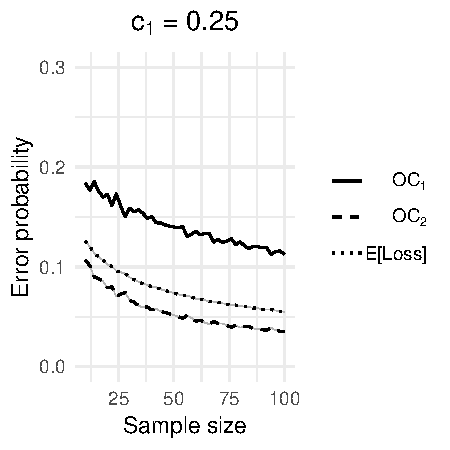
\includegraphics[height=6cm, trim={0 0 2.5cm 0},clip]{./Figures/tiga_c025}
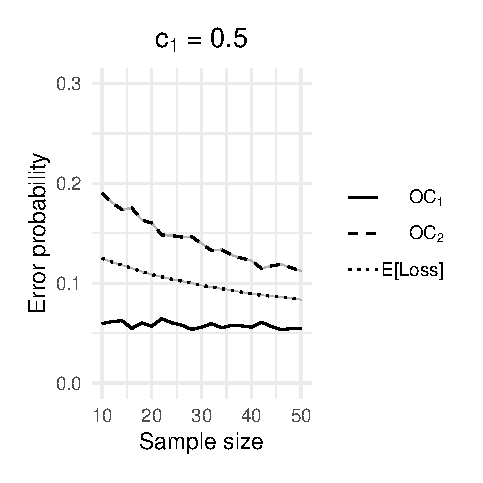
\includegraphics[height=6cm, trim={0.7cm 0 2.5cm 0},clip]{./Figures/tiga_c05}
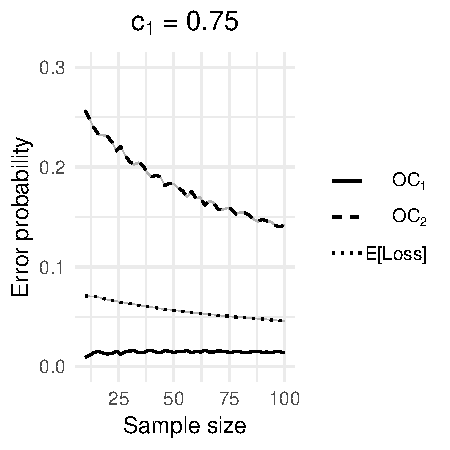
\includegraphics[height=6cm, trim={0.7cm 0 0 0},clip]{./Figures/tiga_c075}
\end{multicols}
\caption{Probabilities of a futile main trial ($OC_1$) and of discarding a promising intervention ($OC_2$) for a range of sample sizes and different values of the loss parameter $c_1$.}
\label{fig:tiga_ocs}
\end{figure}

In Figure~\ref{fig:tiga_n60} we plot the operating characteristics and expected loss obtained as we vary the loss parameter $c_1$ from 0 to 1, whilst keeping the sample size fixed at $n=60$.

\begin{figure}
\centering
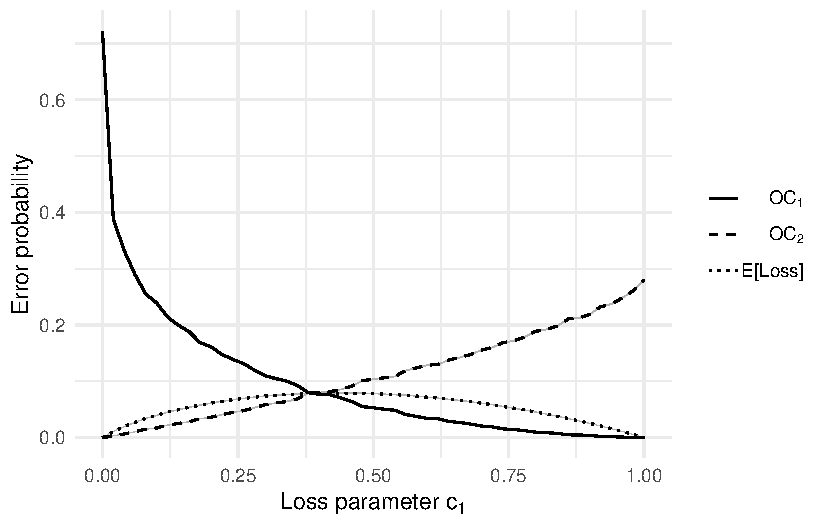
\includegraphics[scale=0.8]{./Figures/tiga_n60}
\caption{Probabilities of a futile main trial ($OC_1$) and of discarding a promising intervention ($OC_2$) for a range of loss parameters $c_1$ when sample size is fixed at $n=60$.}
\label{fig:tiga_n60}
\end{figure}


\section{Illustrative example - Physical activity in care homes (REACH)}\label{sec:REACH}

The REACH (Research Exploring Physical Activity in Care Homes) trial aimed to inform the feasibility and design of a future definitive RCT assessing a complex intervention designed to increase the physical activity of care home residents~\cite{Forster2017}. The trial was cluster randomised at the care home level, with  twelve care homes randomised equally to treatment as usual (TaU) or the intervention plus TaU.

Data on several feasibility outcomes were collected. Here, we focus on four: Recruitment (measured in terms of the average number of residents in each care home who participate in the trial); adherence (a binary indicator at the care home level indicating if the intervention was fully implemented); data completion (a binary indicator for each resident of successful follow-up at the planned primary outcome time of 12 months); and efficacy (a continuous measure of physical activity at the resident level). Progression criteria using the traffic light system were pre-specified for all of these outcomes except efficacy, as shown in Table~\ref{tab:pcs}.

\begin{table}
\caption{Pre-specified progression criteria used in the original REACH design.}
\begin{tabular}{r l l l}
\toprule
Outcome & Red & Amber & Green \\
\midrule
Recruitment & Less than 8 & Between 8 and 10 & At least 10 \\
Adherence & Less than 50\% & Between 50 and 75\% & At least 75\% \\
Follow-up & Less than 65\% & Between 65 and 75\% & At least 75\% \\
\bottomrule
\end{tabular}
\label{tab:pcs}
\end{table}

%The physical activity measure was assumed to be normally distributed with equal variance in each arm, with clustering effects expected due to the intervention being delivered at the care home level. No precise estimates of either the total variance or the intra-cluster correlation coefficient were available, although studies in similar areas did provide some indication of likely values [EXPAND - what likely values?]. The pilot trial led to small samples of data pertaining to both recruitment and delivery, as each is measured at the care home level. In particular, successful delivery could only be assessed at the six care homes in the intervention arm of the trial. 

%Given the proposed pilot design and sample size, we require a method specifying how progression decisions are to be made once the data has been obtained. Given this, we would like to understand the resulting statistical properties of the trial, in terms of how likely we are to make incorrect decisions, and to judge whether or not the pilot will be sufficiently reliable.

\subsection{Model specification}

To begin specifying a model for the REACH trial, we first note that the four substantive parameters can be divided into two pairs. Firstly, mean cluster size and follow-up rate relate to the amount of information which a confirmatory trial will gather. Secondly, efficacy and adherence relate to the effectiveness of the intervention, where effectiveness is thought of as the effect which will be obtained in practice when the effect of non-adherence and other pragmatic effects are accounted for. We expect that a degree of trade-off between adherence and efficacy will be acceptable, with a decrease in one being compensated by an increase in the other. Likewise, low mean cluster size could be compensated to some extent by higher follow-up rate, and vice versa. 

While there may be trade-offs within these pairs of parameters, we do not expect trade-offs between them. A trial with no effectiveness will be futile regardless of the amount of information collected, and so should not be conducted. Similarly, a confirmatory trial should not be conducted if it is highly unlikely to produce enough information for the research question to be adequately answered. We therefore consider the sub-spaces of $\Phi$ formed by these parameter pairs, partition these into hypotheses, and combine these together. Constructing hypotheses in these two-dimensional spaces is cognitively simpler than working in the original four dimensional space, not least because they can be easily illustrated graphically.

Formally, let $\Phi^i$ be the sub-space of mean cluster size and follow-up rate, and $\Phi^e$ be that of adherence and efficacy. Having specified hypotheses $\Phi^i_I, \Phi^e_I$ for $I = R,A,G$, we then have 
\begin{align}\label{eqn:comb_hyp}
\phi \in \begin{cases}
               \Phi_R \text{ if }  \phi^i \in \Phi^i_R \text{ or } \phi^e \in \Phi^e_R \\
               \Phi_G \text{ if }  \phi^i \in \Phi^i_G \text{ and } \phi^e \in \Phi^e_G \\
               \Phi_A \text{ otherwise}. \\
            \end{cases}
\end{align}

\subsubsection{Follow-up and cluster size}

We assume cluster sizes are normally distributed, $m_{i} \sim N(\mu_{c}, \sigma^{2}),~ i = 1 \ldots k$. A normal-inverse-gamma prior 
\begin{equation}
\sigma^{2} \sim \Gamma^{-1} (\alpha_{0}, \beta_{0}), ~ \mu_{c} \sim N(\mu_{0}, \sigma^{2}/\nu_{0})
\end{equation}
is placed on the mean and variance to allow for prior uncertainty in both parameters. It was anticipated that an average of 8 - 12 residents would be recruited in each care home. To reflect this prior belief we set the hyper-parameters to $\mu_{0} = 10, \nu_{0} = 6, \alpha_{0} = 20, \beta_{0} = 39$, giving a prior cluster size of 10 with mean variance 2.05.

We assume that follow up rates are constant across clusters. The number of participants followed-up is assumed to follow a binomial distribution $Bin(\sum_{i=1}^{k} m_{i}, p_{f})$. We take a Beta distribution with hyper-parameters $\alpha_{0} = 22.4, \beta_{0} = 9.6$ as the prior for $p_{f}$. This gives gives a prior with a mean of 0.7 and an effective sample size of 30.

To partition the parameter space into hypotheses, we first consider the case where follow-up is perfect, i.e. $p_{f} = 1$. Conditional on this, we reason that a mean cluster size of below 5 should lead to a red decision (stop development), whereas a size of above 7 should lead to a green decision (proceed to the main trial). As the probability of successful follow-up decreases, we suppose that this can be compensated for by an increase in mean cluster size. We assume the nature of this trade-off is linear and decide that if $p_{f}$ were reduced to 0.8, we would want to have a mean cluster size of at least 8 to consider decisions $a$ or $g$.  We further decide that a follow-up rate of less than $p_{f} = 0.6$ would be critically low, regardless of the mean cluster size, and should always lead to decision $r$. Similarly, a follow-up rate of $0.6 \leq p_{f} < 0.66$ should lead to modification of the intervention or trial design. Together, these conditions lead to the following partitioning of the parameter space:
\begin{equation}
  (p_{f}, \mu_{c}) \in \begin{cases}
               \Phi^i_R \text{ if } p_{f} < 0.6 \text{ or } 20-15p_{f} > \mu_{c} \\
               \Phi^i_G \text{ if } p_{f} > 0.66 \text{ and } 22-15p_{f} < \mu_{c} \\
               \Phi^i_A \text{ otherwise.}
            \end{cases}
\end{equation}

The hypotheses are illustrated in Figure~\ref{fig:hyps} (a). Having specified both the hypotheses and the prior distribution for these two parameters, we can obtain prior probabilities of each hypothesis by sampling from the prior and calculating the proportion of these samples falling into the regions $\Phi^i_R, \Phi^i_A$ and $\Phi^i_G$. We have plotted 1000 samples from the prior in Figure~\ref{fig:hyps} (a), falling into hypotheses  $\Phi^i_R, \Phi^i_A$ and $\Phi^i_G$ in proportions 0.354, 0.517, 0.129 respectively. This demonstrates that there is significant prior uncertainty regarding the optimal decision, indicating the potential value of the pilot trial.

\begin{figure}
   \centering
   \subfloat[][]{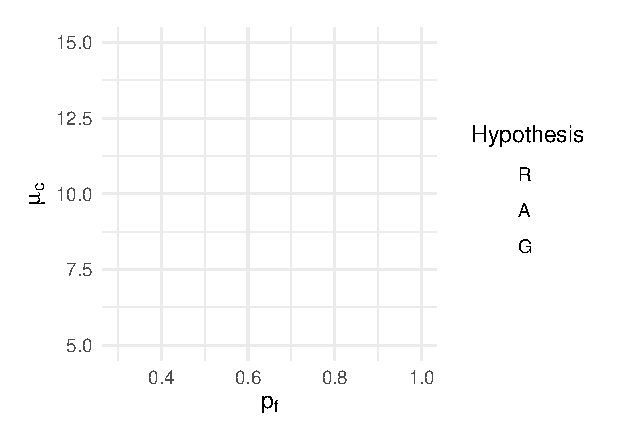
\includegraphics[height=4.4cm, trim={0 0 2.8cm 0},clip]{./Figures/hyp_fu_cl}}\quad
   \subfloat[][]{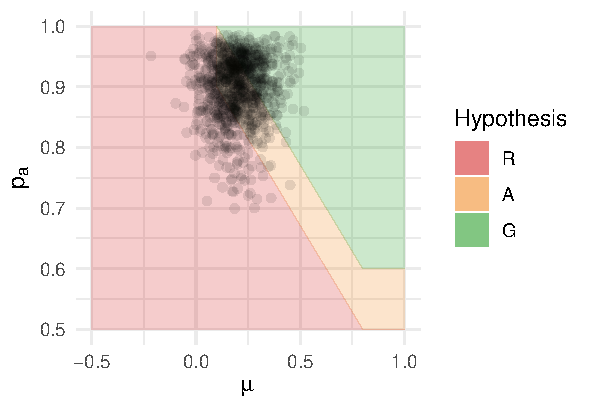
\includegraphics[height=4.4cm]{./Figures/hyp_ad_eff}}\\
   \caption{Marginal hypotheses over parameters for (a) follow-up rate $p_{f}$ and mean cluster size $\mu_{c}$; and (b) adherence rate $p_{a}$ and efficacy $\mu$. Each point is a sample from the joint prior distribution.}
   \label{fig:hyps}
\end{figure}

\subsubsection{Adherence and efficacy}

Having defined priors and hypotheses with respect to cluster size and follow-up, we now consider adherence and efficacy. The number of care homes which successfully adhere to the intervention delivery plan is assumed to be binomially distributed with probability $p_{a}$. We assume that adherence is absolute in the sense that all residents in a care home which does not successfully deliver the intervention will not receive any of the treatment effect. We place a Beta prior on $p_{a}$, with hyper-parameters $\alpha = 28.8$ and $\beta = 3.2$ giving a prior mean of 0.9 from an effective sample size of 32.

The continuous measure of physical activity is expected to be correlated within care homes. We model this using a random intercept, where the outcome $y_{i,j}$ of resident $i$ in care home $j$ is
\begin{equation}
y_{ij} = X_{j} \times Y_{j} \times \mu + u_{j} + \varepsilon_{i}.
\end{equation}
Here, $X_{j}$ is a binary indicator of care home $j$ being randomised to the intervention arm, $Y_{j}$ is a binary indicator of care home $j$ succesfully adhering to the intervention, $u_{j} \sim \mathcal{N}(0, \sigma_{B}^{2})$ is the random effect for care home $j$ and $\varepsilon_{i} \sim \mathcal{N}(0, \sigma_{W}^{2})$ is the residual for resident $i$. We parametrise the model using the intracluster correlation coefficient $\rho = \sigma_{B}^{2} / (\sigma_{B}^{2} + \sigma_{W}^{2})$, and place priors on $\mu, \rho$, and $\sigma_{W}^{2}$ in the manner suggested in~\cite{Spiegelhalter2001}. Specifically, we choose
\begin{align}
\mu & \sim N(0.2, 0.25^{2}) \\
\sigma_{W}^{2} & \sim \Gamma^{-1}(50, 45) \\
\rho & \sim Beta(1.6, 30.4).
\end{align}
To reflect prior expectation of an ICC around 0.05 but possibly as large as 0.1, the hyperparameters give a prior mean of 0.05 for the ICC with a prior probability of 0.104 that it will exceed 0.1. 

We consider that while there is potential for adherence to be improved after the pilot, there will be little opportunity to improve the efficacy of the intervention. Moreover, we suppose an absolute improvement in delivery of up to around 0.1 is feasible. To define the hypotheses in this subspace we first set a minimal level of efficacy to be 0.1, and decide that we would be happy to make decision $g$ at this point if and only if adherence is perfect. As $p_{a}$ reduces from 1, a corresponding linear increase in efficacy is considered to maintain the overall effectiveness of the intervention. The rate of substitution for this trade-off is determined to be approximately 0.57 units of efficacy per unit of adherence probability. We consider an absolute lower limit in adherence of $p_{a} = 0.5$, below which we will always consider decision $r$ to be optimal. Taking these considerations together, the marginal hypotheses are defined as

\begin{equation}
  (p_{a}, \mu) \in \begin{cases}
               \Phi^e_R \text{ if } p_{a} < 0.5 \text{ or } 0.96-0.57\mu > p_{a} \\
               \Phi^e_G \text{ if } p_{a} > 0.6 \text{ and } 1.06-0.57\mu < p_{a} \\
               \Phi^e_A \text{ otherwise.}
            \end{cases}
\end{equation}

The hypotheses are illustrated in Figure~\ref{fig:hyps} (b). Again, a sample of size 1000 from the joint marginal prior distribution $p(p_{a}, \mu)$ is also plotted, falling into hypotheses $\Phi^e_R, \Phi^e_A$ and $\Phi^e_G$ in proportions 0.234, 0.470, 0.296 respectively. As before, this indicates substantial prior uncertainty regarding the optimal decision and thus supports the use of a pilot study.

The marginal hypotheses are combined together using equation (\ref{eqn:comb_hyp}). Considering the same 1000 samples from the design prior plotted in Figure~\ref{fig:hyps}, these now fall into the regions $\Phi_R, \Phi_A$ and $\Phi_G$ in proportions 0.507, 0.458, and 0.035 respectively. Note that the prior probabilities of these overall hypotheses are quite different to those of the marginal hypotheses. In particular, there is a considerable increase in the probability that decision $r$ will be optimal, and a considerable decrease that decision $g$ will be.

\subsection{Evaluation and optimisation}

\subsubsection{Weakly informative analysis}

We applied the proposed method assuming that a weakly informative joint prior distribution will be used at the analysis stage\footnote{Full details of the weakly informative prior are given in the appendix.}. We took the sample size of the trial to be $k = 12$ clusters, randomised equally between arms. For calculating operating characteristics we generated $N = 10^4$ samples from the joint distribution $p(\theta, x) = p(x | \theta)p_D(\theta)$. We analysed each simulated data set using Stan via the R package rstan~\cite{rstan}, in each case generating 5000 samples in four chains and discarding the first 2500 samples in each to allow for burn-in, leading to $M = 10^4$ posterior samples in total. This gave a maximum Monte Carlo error of approximately 0.005 when estimating a posterior probability $Pr[\phi \in \Phi_I ~|~ x]$, which we considered sufficient. These posterior samples were then used to find the posterior probabilities of each hypothesis, for each simulated data set.

%For each of the $N$ samples $(\theta^{(i)}, x^{(i)})$ we extracted the estimated posterior probabilities $p_R$ and $p_G$, plotted in Figure~\ref{fig:post_probs}. We observe a large mass of points with very low values of $p_G$ and high values of $p_R$. These can be contrasted with the prior probability of each hypothesis, with respect to the design prior $p_D(\theta)$. The majority of simulated data sets lead to a movement from the prior point to a larger value of $p_R$, suggesting the analysis is being conservative.

%\begin{figure}
%\centering
%\includegraphics[scale=0.8]{./Figures/post_probs}
%\caption{Posterior probabilities $(p_{R}, p_{G})$ of $N = 10^4$ simulated pilot data sets. The prior probability taken from the design prior $p_D$ is shown in red.}
%\label{fig:post_probs}
%\end{figure}

We evaluated the operating characteristics for a sample of parameters $(c_1, c_2, c_3)$ as described in Section~\ref{sec:optimisation}. A total of 249 parameter vectors were evaluated, of which 193 led to operating characteristics which were worse in every respect than some other vector (i.e. dominated) and thus were discarded. The operating characteristics of the non-dominated parameters are shown in Figure~\ref{fig:p_front}. The three operating characteristics are found to be highly correlated. In particular, changing the parameters to give a lower probability of discarding a promising intervention ($OC_2$) tends to lead to a reduction in the probability of making an unnecessary adjustment ($OC_3$). When selecting $(c_1, c_2)$, the key decision appears to be trading off the probability of a futile trial, ($OC_{1}$), against $OC_{2}$. There is a very limited opportunity to minimise $OC_{3}$ at the expense of these. For example, compare points $b$ and $c$ in Figure~\ref{fig:p_front}, details of which are given in Table~\ref{tab:costs}. We see that point $c$ reduces $OC_3$ by 0.049 in comparison to point $b$, but only at the expense of increase in $OC_1$ and $OC_2$ of 0.105 and 0.072 respectively.

\begin{figure}
\centering
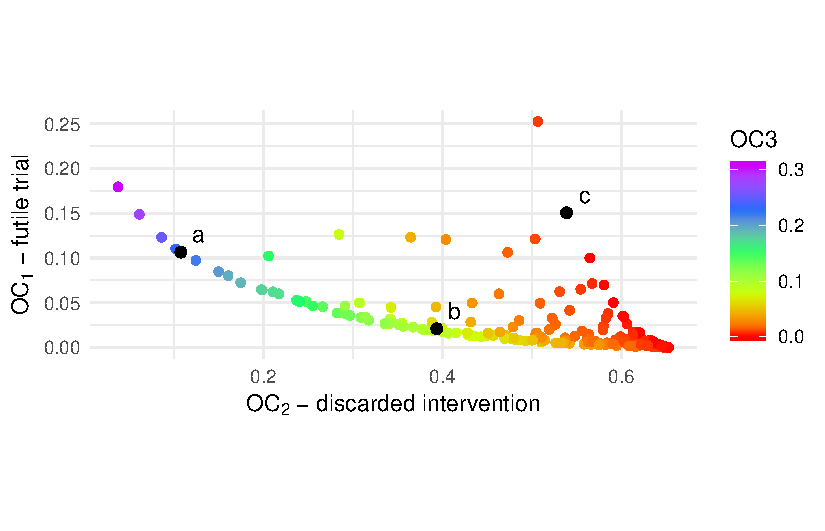
\includegraphics[scale=0.8]{./Figures/p_front}
\caption{Operating characteristics of the example pilot trial for a range of loss parameter vectors, when a weakly informative analysis prior is used.}
\label{fig:p_front}
\end{figure}

\begin{table}
\caption{Estimated operating characteristics (with standard errors) of the REACH trial for the three loss parameter vectors highlighted in Figure~\ref{fig:p_front}, when a weakly informative analysis prior is used. Costs have been rounded to 2 decimal places; operating characteristics and their errors to 3.}
\begin{tabular}{r l l l l}
\toprule
Label & $(c_{1}, c_{2}, c_{3})$ & $OC_{1}$ & $OC_{2}$ & $OC_{3}$ \\
\midrule
$a$ & (0.14, 0.85, 0.02) & 0.165 (0.004) & 0.096 (0.003) & 0.204 (0.004) \\
$b$ & (0.32, 0.57, 0.10) & 0.047 (0.002) & 0.287 (0.005) & 0.078 (0.003)  \\
$c$ & (0.03, 0.52, 0.45) & 0.152 (0.004) & 0.359 (0.005) & 0.032 (0.002)  \\
\bottomrule
\end{tabular}
\label{tab:costs}
\end{table}

We may expect to see a clear relationship between the value of parameters $c_1, c_2, c_3$ and the operating characteristics they relate to. We explore this in Figure~\ref{fig:cost_OCs} with scatter plots of each  parameter against each operating characteristic. The results show that there is indeed a strong relationship between the loss assigned to discarding a promising intervention, $c_2$, and the probability that this event will occur (see bottom right plot). Moreover, $c_2$ also seems to be the main determinant of operating characteristics $OC_1$ and $OC_3$. The implication is that once the $c_2 \in [0,1]$ has been chosen, the operating characteristics of the trial depend only weakly on the way in which the remaining $1-c_3$ is allocated to $c_1$ and $c_3$. This appears to be due to the fact that, regardless of how errors are weighted, the way we have defined our prior distributions and hypotheses means we are much more likely to make the error of discarding a promising intervention than the other types of error. The cost we assign to this error is therefore more influential on the overall operating characteristics than the other costs.

\begin{figure}
\centering
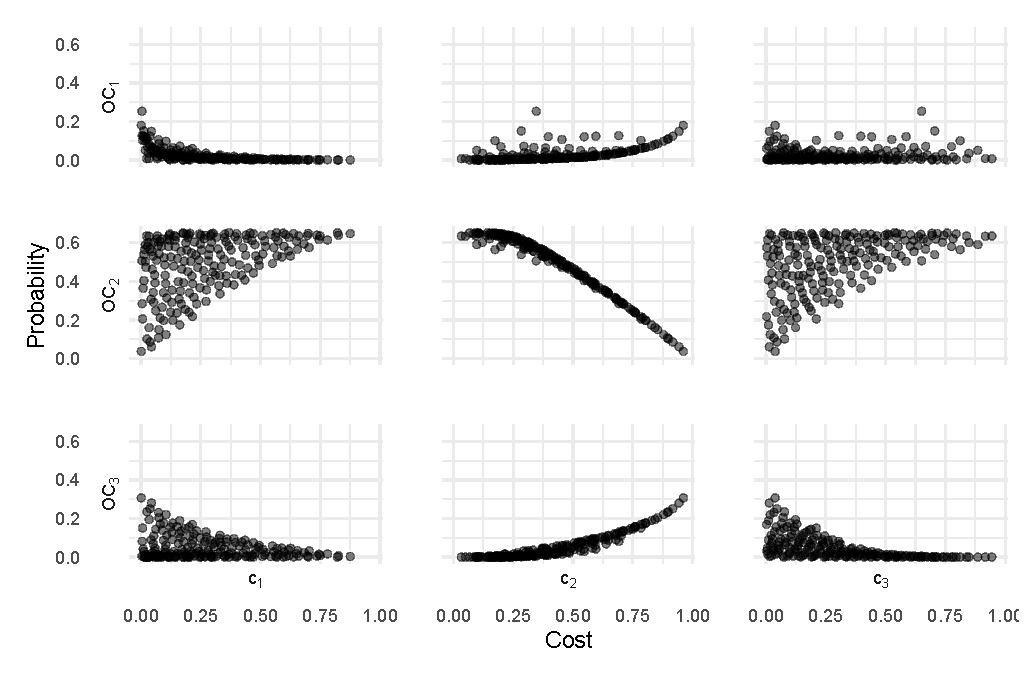
\includegraphics[scale=0.8]{./Figures/cost_OCs}
\caption{Relationships between the three loss parameters ($x$ axes) and resulting operating characteristics ($y$ axes).}
\label{fig:cost_OCs}
\end{figure}

\subsubsection{Incorporating subjective priors}

Rather than use weakly or non-informative priors when analysing the pilot data, we may instead want to make use of the (subjective) knowledge of parameter values that was elicited and described in the design prior $p_D(\theta)$. Anticipating criticisms of a fully subjective analysis, we can envisage two particular cases where this might be appropriate. Firstly, using the components of the design prior which describe the nuisance parameters $\psi$ while maintaining weakly informative priors on substantive parameters $\phi$. Secondly, when very little data on a specific substantive parameter is going to be collected in the pilot, using the informative design prior for that parameter could substantially improve operating characteristics.

We replicated the above analysis for these two scenarios. For the second, we used informative priors for all nuisance parameters and for the probability of adherence, $p_a$. Recall that this is informed by a binary indicator for the 6 care homes in the intervention arm, and will therefore have very little pilot data bearing on it. For each case we used the same $N$ samples of parameters and pilot data which were used in the weakly informative case, repeating the Bayesian analysis using the appropriate analysis prior and obtaining estimated posterior probabilities $p_R, p_A$ and $p_G$ as before. These were used in conjunction with the same set of loss parameter vectors $\mathcal{C}$ to obtain corresponding operating characteristics.

For brevity we will refer to the three cases as Weakly Informative (WI), Informative Nuisance (IN), and Informative Nuisance and Adherence (INA). Comparing the operating characteristics of cases WI and IN, we found very little difference (further details are provided in the appendix). When we contrast cases WI and INA, however, there is a clear distinction. Using the INA analysis prior will lead to larger probabilities of a futile trial ($OC_1$) and of unnecessary adjustment ($OC_2$), while reducing the probability of discarding a promising intervention ($OC_3$), for almost all loss parameters. The expected loss is always lower for the INA analysis than for WI, as we would expect. Further details can be found in the appendix.

%Although the posterior distributions $p(\theta | x)$ are qualitatively different when we examine an individual sample of pilot data, these differences do not translate to the posterior probabilities of hypotheses.

%\begin{figure}
%\centering
%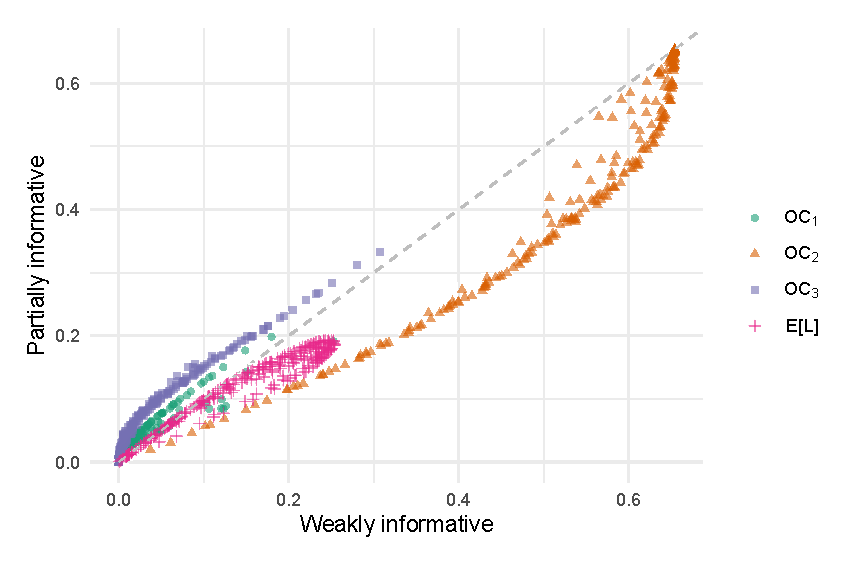
\includegraphics[scale=0.8]{./Figures/an_prior_comp}
%\caption{Operating characteristics and expected utilities for weakly (WI) and partially informative (INA) %analyses. Each point represents a different cost vector.}
%\label{fig:an_prior_comp}
%\end{figure}

\section{Discussion}\label{sec:discussion}

%In fact, hypothesis testing is generally discouraged due to concerns that the analysis will be under-powered~\cite{Lancaster2004, Arain2010, Thabane2010}.

%While there is a considerable literature on statistical approaches to pilot design when the aim of the pilot is to estimate a parameter that will be used in the sample size calculation of the main RCT, 

%Note that we do not need to elicit an axact value of $c$ to make our decision. Once $Pr[ \phi \in \Phi_G ]$ has been calculated, we only need to decide if our $c$ is less than this value in order to know that proceeding is the optimal action. We are just choosing between two gambles. On the one hand, we can choose $g$ and make a type I error with $1 - Pr[ \phi \in \Phi_G ]$, or we can choose $r$ and make a type II error with $Pr[ \phi \in \Phi_G ]$. 

When deciding if and how a definitive RCT of a complex intervention should be conducted, and basing this decision on an analysis of data from a small pilot trial, there is a risk we will inadvertently make a poor choice. A Bayesian analysis of pilot data followed by decision making based on a loss function can help ensure this risk is minimised. The expected results of such a pilot can be evaluated through simulation at the design stage, producing operating characteristics which help us understand the potential for the pilot to lead to better decision making. These evaluations can in turn be used to find the loss function which leads to the most desirable operating characteristics, avoiding the need for any direct elicitation of decision maker preferences, and to inform the choice of sample size.

Our proposal has been motivated by some salient characteristics of complex intervention pilot trials, and offers several potential benefits over standard pilot trial design and analysis techniques. The Bayesian approach to analysis means that complex multi-level models can be used to describe the data, even when the sample size is small. In contrast to the usual application of independent progression criteria for several parameters of interest, we provide a way for preferential relationships between parameters to be articulated and used when making decisions. Using a subjective prior distribution on unknown parameters at the design stage allows both our knowledge and our uncertainty to be fully expressed, meaning we can leverage external  information whilst also avoiding decisions which are highly sensitive to imprecise parameter estimates.

Our proposed design is related to the literature on assurance calculations for clinical trials, applying the idea of using unconditional event probabilities as operating characteristics to the pilot trial setting. In doing so we have defined assurances on multiple substantive parameters and with respect to the `traffic light' red/amber/green decision structure. The multi-objective optimisation framework we have used to inform trial design avoids setting arbitrary thresholds for operating characteristics as are commonly seen, and criticised~\cite{Bacchetti2010}, with type I and II error rates.

The benefits brought by the Bayesian approach must be set against the challenges it brings, particularly in terms of computation time and implementation. In terms of the latter, we are required to specify a joint prior distribution over the parameters $\theta$ and a partitioning of the parameter space into the three hypotheses. The specification of the prior distribution may be a challenging and time-consuming task. Although some relevant data relating to similar contexts may be available, for example in systematic reviews or observational studies, expert opinion may still be required to articulate the relevance of such data to the problem at hand. When no data are available, which is not unlikely given the early phase nature of pilot studies, expert opinion will be the only source of information. Although potentially challenging, many examples describing successful practical applications of elicitation for clinical trial design are available~\cite{Walley2015, Crisp2018, Dallow2018}, as are tools for its conduct such as the Sheffield Elicitation Framework (SHELF)~\cite{OHagan2006a}. Dividing the parameter space into three hypotheses may also prove challenging in practice, particularly when trade-offs between more than two parameters are to be elicited. There is a need for methodological research investigating how methods for multi-attribute preference elicitiation, such as those set out in~\cite{Keeney1976}, can be applied in this context. 

%To minimise the burden, the statistical model should be constructed where possible to ensure the parameters can be considered independent~\cite{OHagan2012}, thus allowing the full joint distribution to be defined as the product of the individual priors.  

The computational burden of the proposed method is significant, particularly when the model is too complex to allow a simple conjugate analysis to be used when sampling from the posterior distribution. We have used a nested Monte Carlo sampling scheme to estimating operating characteristics, as seen elsewhere~\cite{Wang2002, OHagan2005, Sutton2007}. One potential approach to improve efficiency is to use non-parametric regression to predict the expected losses of Equation (\ref{eqn:exp_loss}) based on some simulated data, thus bypassing the need to undertake a full MCMC analysis for each of the $N$ samples in the outer loop. This approach has been shown to be successful in the context of expected value of information calculations~\cite{Strong2014, Strong2015}. The computational difficulties will be particularly pertinent when using our approach to choose determine sample size, where several evaluations of different choices will be required. If the choice of sample size can be framed as an optimisation problem, methods for efficient global optimisation of computationally expensive functions such as those described in~\cite{Jones2001, Roustant2012} may be useful~\cite{Wilson2015}.

%We have not considered how to choose the optimal sample size of a pilot trial in this paper. The standard approach is to refer to one of many rules-of-thumb, such as those described in~\cite{Lancaster2004, Julious2005, Teare2014}, although the shortcomings of such a one-size-fits-all approach have been highlighted~\cite{Whitehead2015}. While our framework could be used to assess the operating characteristics of several choices of sample size, the aforementioned computational burden of each assessment will make this difficult in practice. However, the small samples typically available for pilot trials suggests that such optimisation may not be crucial. When it is deemed necessary, methods developed for the design and analysis of expensive computer experiments may provide a way for it to be conducted in an efficient manner~\cite{Jones2001}.

%The standard approach to the analysis of pilot trials involves pre-specifying some progression criteria for the parameters of interest, and basing decisions (at least in part) on whether or not parameter estimates satisfy these criteria. This framework specifies a decision rule mapping the pilot data to decisions, as we have done in this paper, but does so implicitly and with no statistical analysis of the resulting properties. An alternative approach would be to employ formal hypothesis tests under a frequentist view. This would have the advantage of not requiring a joint prior distribution to be specified when designing the pilot. However, there has been limited reaseach into how preferential relations between parameters can be incorporated into such testing procedures, typically focussing on the case of two parameters~\cite{Conaway1996, Thall2008}. Moreover, testing multiple parameters can lead to multiplicity. In the case of union tests, type I error rate can be inflated; whilst in the case of intersection tests, type II error rate can be inflated~\cite{Senn2007}. Hybrid approaches which assume a freqentist analysis but take a Bayesian view to design by averaging type I~\cite{Chuang-Stein2007} or type II~\cite{Spiegelhalter1986} error rates have been proposed, and may go some way to addressing these issues.

We have defined our procedure in terms of a loss function, where the decision making following the pilot will minimise expected loss. However, the piecewise constant loss function we have proposed may not adequately represent the preferences of the decision maker. For example, we may object to the loss associated with discarding a promising intervention being independent of how effective the intervention is. An alternative is to try to define a richer representation of the loss function through direct elicitation of the decision makers preferences under uncertainty~\cite{French2000}, leading to a fully decision-theoretic approach to design and analysis~\cite{Lindley1997}. However, as previously noted by others~\cite{Joseph1997a, Bacchetti2008, Whitehead2008}, implementation of these approaches has been limited in practice and may be indicative of their feasibility.

%We have suggested that the loss function can be parametrised with respect to the operating characteristics it produces. While this is a common strategy when implementing decision-theoretic approaches to trial design~\cite{Lewis2007}, an alternative is to define the loss function through direct elicitation of the decision makers preferences under uncertainty~\cite{French2000}. This leads to a fully decision-theoretic approach to design and analysis~\cite{Lindley1997}. 

%Our discussion has also glossed over the difference between a loss function and a value function, where the former is defined strictly with respect to uncertainty and should encode an attitude to risk, while the former considers preferences under conditions of certainty and is not relevant to taking expectations~\cite{French2000}. 

%Instead of basing decisions on the expected value of a loss function, a decision rule based directly on posterior probabilities could be used, as in e.g. \cite{Chen2011a, Cellamare2014, Ibrahim2014}. If employing the optimisation approach described in Section~\ref{sec:optimisation} this would make no difference, but if defining the decision rule directly it is possible that this could be easier to do in terms of posterior probabilities than in terms of the cost parameters of the loss function.

% elaborate on the inadequacy of our loss function. Not just that its piecewise constant, but also think about value, utlity, and attitude to risk. Principle of maximising expected utility only applies if our utility function is defined in an uncertain context, i.e. utility reflects preferences between gambles. Perhaps not relevant when we are fitting the loss function to OCs?
 

% extensions

The proposed method could be extended in several ways. For example, more operating characteristics could be defined and used in design optimisation, more complicated trade-off relationships between multiple parameters could be addressed, or the hypotheses could be expanded to include nuisance parameters which would be used as part of the sample size calculation in the main RCT. A particularly interesting avenue for future research is to consider how  to model post-pilot trial actions in more detail. For example, while we allow for the possibility of making an `amber' decision, indicating that modifications to the intervention or trial design should be made, we do not model what that decision will actually look like. The type of amber adjustments needed are very different in different parts of the hypothesis space, and so we may attempt to improve recruitment rate (for example) when in fact it is adherence which requires improvement. Methodology for jointly modelling a pilot and subsequent main RCT in this manner could be informed by developments for designing phase II/III programs in the drug setting ~\cite{Stallard2012, Goette2015, Kirchner2015}.

%This points to a significant challenge in pilot trials - the difficulty in modelling post-trial action, the richness of the decision space. Contrast with the drug setting where nothing much changes, and we just decide on a phase III sample size. Hence plenty papers looking at optimising the whole process, not just the phase II trial itself. An example of modelling the change is the internal pilot assessing recruitment in~\cite{Hampson2017}.

%Different OCs

%More expansive hypothesis space:
%- including nuisance parameters
%- more complex trade-offs e.g. > 2 parameters, elicitation challenges

%Modelling:
%- design of main RCT using pilot information (e.g. ICC or SD distribution)
%- changes between pilot and main RCT
%- health economics after main RCT

%Some of the literature on pilot studies focusses not on progression decisions, but on generating information on one or more parameters that will be used for the main trial sample size calculations, e.g. \cite{Browne1995}. NIHR guidance on pilots says that ``the sample size should be adequate to estimate the critical parameters (e.g. recruitment rate) to the necessary degree of precision''~\cite{NIHR2017}. But \cite{Eldridge2015} shows that getting a point estimates of an ICC from a pilot and using it in the main trial sample size calculation is not a good approach due the substantial sampling variation of the estimate. Several papers have demonstrated the potential benefits of designing a trial using a prior on the ICC to properly encapsulate knowledge and uncertainty e.g. \cite{Spiegelhalter2001}, \cite{Turner2004}. Our approach will lead to distributions on all parameters, including the ICC, and so could feed in directly to these approaches. \cite{Eldridge2006} - ``A Bayesian approach to analysis in which the ICC is determined by a prior distribution as well as the trial data itself may alleviate the problem of uncertainty in predicting the ICC.''. More generally, many papers have shown how to use assurance calculations when designing the main RCT, and our approach would provide the distribution over parameters that these methods average over.

%We have not specifically considered the issue of choice of sample size for the pilot study, instead assuming that this will primarily be chosen with respect to logistical and financial constraints. Nevertheless, the evaluation we propose could be applied to several possible choices of sample size, allowing the cost of increased sampling to be explicitly weighed against the resulting improvement in operating characteristics. Although the method is computationally expensive as we would need to run the full nested simulation routine for each new sample size, the inherently restricted size of a pilot will mean we don't have many options to consider so this may not be prohibitive. Even without a comparison of different sample sizes, our method allows us to understand the quality of the typical default sample size suggestions as given in~\cite{Lancaster2004, Browne1995}\footnote{As previously discussed, this rule seems to have been born out of a mis-reading of the Browne paper - he actually advised against using this rule-of-thumb.}, \cite{Julious2005} and~\cite{Teare2014}.

%``the sample size should be adequate to estimate the critical parameters (e.g. recruitment rate) to the necessary degree of precision''~\cite{NIHR2017}
%``our results show that most estimates of rates for pilots of cluster randomised trials are likely to be subject to considerable uncertainty so we suggest researchers need to be cautious about setting definitive thresholds that may then be missed by chance'' ~\cite{Eldridge2015}

% Limitations

%We do not model the larger evaluation process, i.e. we consider only the pilot. An alternative would be to jointly model the early and late phase trials. See a lot in phase II / III setting, e.g. \cite{Stallard2012} or \cite{Goette2015} or \cite{Kirchner2015}. But clearly more complex for us. Note that pilots are the topic in~\cite{Whitehead2015}, but their problem is much simpler - just estimating a standard deviation. More modelling could also encapsulate health economics, connecting with EVI literature~\cite{Strong2014, Strong2015}.


\bibliographystyle{unsrt}
\bibliography{U:/Literature/Databases/DTWrefs}

\end{document}